\section{Demonstrations}
\label{sec:demo}

The scenario where the COACHES robots and systems will be deployed, demonstrated, and validated is provided by the mall ``Rives de l'Orne''\footnote{\url{http://www.rivesdelorne.com}}, located in the city of Caen, France  (see Fig. \ref{fig:outsidemall}).

\begin{figure}[!t]
\begin{center}
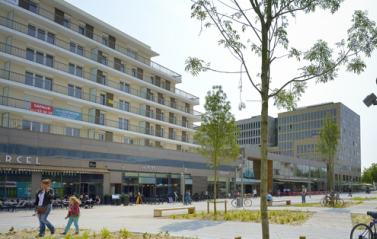
\includegraphics[width=0.55\linewidth]{fig/outsiderivesdelorne}
\caption{The mall Rives de l'Orne.}
\label{fig:outsidemall}
\end{center}
\end{figure}

\begin{figure}[htbp]
\begin{center}
\includegraphics[height=5cm]{fig/MapsRorne}
\caption{The map}
\label{fig:map}
\end{center}
\end{figure}

\begin{figure}[htbp]
\begin{center}
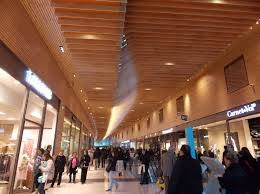
\includegraphics[height=6cm]{fig/InsideRivedelOrne}
\caption{Inside the mall}
\label{fig:insidemall}
\end{center}
\end{figure}

The test facility is a new and modern mall composed of two face-to-face buildings separated by a large main square. Figure \ref{fig:map} shows a plan of the mall.
At the first floor of the two buildings, there are many shops and restaurants (as shown in Figure \ref{fig:insidemall}). In the main square, there is a cinema. This space is surrounded by tramway stations and a train station. This mall is visited by more than 100,000 customers every year. In addition to that, several elderly people live in the new apartments at the other floors of the buildings. These people have their habit and there are frequent customers of the mall. 

Two meetings have been organized ($23^{th}$ October and $12^{th}$ December 2014) to define the equipments to install in terms of sensors.

Cameras and other sensors are in charge of sending information to the COACHES robots about the environment.
%\begin{itemize}
%\item the shops;
%\item the planning of the robot deployment in the mall;
%\item the scheduled dissemination actions.
%\end{itemize}
Moreover, Radio-Frequency IDentification (RFID) tags and receivers could be used to identify shops and possibly key people for the application.

The shopping mall is a perfect environment to test and validate the use cases described in the previous section. Some of them will be thus fully implemented and tested with real customers of the shopping mall, within the course of the project.



\subsection{Testing the use cases}

The use cases described above will be tested in the shopping mall of Caen with the following procedure.
\begin{enumerate}
\item Description to shop keepers and managers to collect feedback and apply modifications or provide more details.
\item Test with real users using a mock-up implementation where the robot is driven by a user operator.
\item Implementation and test of the fully autonomous behavior in an incremental way, by allowing at intermediate phases the use of non-fully autonomous components.
\item Final test of the fully autonomous behaviors with real users.
\end{enumerate}



